\section{Tasks for AVs}\label{sec:probAnal-tasksAV}
This section will elaborate on which problems or tasks an AV system needs to address in order to be operational.
The purpose of this is to make an overview of specific technical problems pertaining to the development of a functional AV system.

If the purpose of an AV is to replace a human driver, it should as a minimum be able to do the same job as effectively and safely as the average human driver.
There are several tasks involving this overall objective.
The AV needs to be able to sense its environment and interpret this, as well as make the necessary planning and decisions to reach its goal destination safely.
An overview of a general AV system can be seen in \autoref{fig:AV_System}.
It consists of hardware and software, which are used to perceive and make decisions in its environment.

\begin{figure} [H]
    \centering
    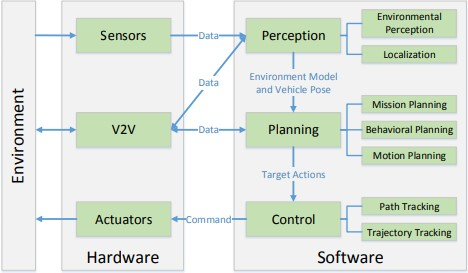
\includegraphics{AV_Model.jpg}
    \caption{Overview of a general AV system \cite{pendleton_perception_2017}}
    \label{fig:AV_System}
\end{figure}

The hardware is the components used to gather data about the environment, such as cameras, Light Detection and Ranging (LiDAR)\footnote{LiDAR is used to create a three-dimensional map of the environment using the reflections of light pulses being sent out \cite{pendleton_perception_2017}.}, GPS, infrared sensors, etc.
Other hardware components are Vehicle-to-Vehicle (V2V) communication and the actuators, such as vents on the car, the motor, etc.

The software components, as seen in \autoref{fig:AV_System}, interact with the hardware in order for it to \textit{perceive} its environment, \textit{plan} its actions and \textit{control} the actuators according to the plans.
These three software components are elaborated on further in the following subsections.

\subsection{Perception}\label{ssec:tasksForAVs-Perception}
During the perception task, the AV system starts the process of understanding the data, and changing it into something it can use to make decisions.
The objective is to make a model of the environment.
This is where the AV system identifies objects, such as pedestrians and other cars.
In addition to identifying objects, the AV system must also understand the space it moves within, e.g. by keeping track of the car's position, both in its current lane, on a global scale, as well as keeping track on how close different objects are to the vehicle.
In a simple setting, the perception task could be just to model the car's position and orientation in relation to the road lanes.
The result of the perception component should be a sufficient model of the environment (including the vehicle's position), which will then be used by the planning component in order to plan its actions.
\cite{pendleton_perception_2017}

\subsection{Planning}
Once the AV system has processed the raw data into something it can understand, it needs to make decisions based on this information.
This includes immediate decisions, such as stopping for red lights or making lane changes, or more long term decisions, such as planning the best route to drive.
\cite{pendleton_perception_2017}

\subsection{Control}
This is where the plans are actualized by converting them into actual commands for the car, e.g. what angle do the wheels need to be at, or how fast should the vehicle drive.
\cite{pendleton_perception_2017}
